\part{Análisis de requisitos}
\section{Introducción}

\subsection{Requisito}
 Condiciones o capacidades de debe cumplir un sistema para satisfacer un contrato, norma o especificación.
 
\subsubsection{Clasificación de los requisitos}
\begin{itemize} % Para llamarlos así mejor requisitos declarativos, restrictivos y de dominio... estan como el rabo quiere
    \item \textbf{Requisitos funcionales}: Declaraciones de los servicios o funcionalidades que implementará el sistema. \textit{Ejemplo: El usuario tendrá la posibilidad de buscar por tamaño}.
    
    \item \textbf{Requisitos no funcionales}: Restricciones sobre los servicios o funciones ofrecidos por el sistema. Pueden ser temporales, de fiabilidad, robustez, de ajuste a estándares\ldots\\
    Deben expresarse de forma cuantitativa. 
    \textit{Ejemplo: La duración de la sesión ha de ser superior a 30 minutos}.
    
    \item \textbf{Requisitos del dominio}: Provienen del entorno en el que se realiza la aplicación y pueden ser funcionales o no funcionales. \textit{Ejemplo: usar el formato DICOM en medicina es a la vez un requisito no funcional y de entorno}.
\end{itemize}

\subsection{Análisis de requisitos}

Proceso de \textbf{estudio de las necesidades de los usuarios} para llegar a una definición de los requisitos obtenidos, incluyendo el proceso de refinamiento de los mismos.
\\\\
Encontramos este proceso en todos los modelos de ciclos de vida, compartiendo las siguientes características comunes:
\begin{enumerate}
    \item Realizan una abstracción de las características del sistema.
    \item Representan el sistema de forma jerárquica.
    \item Definen las interfaces del sistema, tanto externas como internas. %definen las interfaces internas entre modulos pero en esta fase todavía no se crearon módulos, bien rabenso.
    \item Sirven de base para etapas posteriores del diseño e implementación.
    \item Se plantean por niveles: usuario, de sistema, esenciales y de implementación.
    \item No prestan demasiada atención a la representación de las restricciones o criterios de validación. (excepto los métodos formales).
\end{enumerate}

\textit{Rabenso dice: Por norma general, se debería dedicar un 40\% del tiempo de desarrollo de un proyecto al análisis y diseño, un 20\% a la codificación, y un 40\% a la fase de pruebas.}

\subsection{Personal implicado}

\begin{enumerate}
\item \textbf{Analista}: Es el encargado de la comunicación con los stakeholders y los desarrolladores, sirviendo de puente entre ambos. Para este labor debe de tener conocimiento multidisciplinar, buenas dotes de comunicación y ser capaz de traducir ideas vagas de necesidades de software en un conjunto concreto de funciones y restricciones.

\item \textbf{Stakeholders}: personal involucrado en el proyecto, incluyendo a los usuarios finales, los ingenieros trabajando en el proyecto, el administrador de negocio y los expertos del dominio del sistema. Podemos distinguir entre involucrados y comprometidos.
\end{enumerate}


\subsection{Razones por las que el análisis de requisitos es difícil}
\textit{Sommerville} establece las siguientes razones:
\begin{itemize}
    \item Los stakeholders a menudo no conocen realmente lo que desean obtener del sistema.
    \item Los stakeholders expresan los requisitos con sus propios términos. Los ingenieros de requisitos deben comprenderlos.
    \item Diferentes stakeholders tienen requisitos distintos que expresan de varias formas. Los ingenieros de requisitos tienen que descubrir todas las fuentes potenciales de requisitos así como las partes comunes y en conflicto.
    \item Puede haber condicionantes políticos y de la organización.
    \item El entorno económico y de negocios en el que se lleva a cabo el análisis es dinámico, y cambia durante el proceso de análisis, por lo que la importancia de ciertos requisitos puede cambiar.
\end{itemize}


\section{Obtención de requisitos} %Sigamos la convención del rabenso
El proceso de análisis de requisitos tiene las siguientes fases:
\begin{itemize}
    \item \textbf{Identificar las fuentes de información} relevantes para el proyecto.
    \item \textbf{Realizar las preguntas apropiadas} para comprender sus necesidades.
    \item \textbf{Analizar la información recogida} para detectar aspectos poco claros.
    \item \textbf{Confirmar con los usuarios} lo que se ha comprendido de los requisitos.
    \item \textbf{Sintetizar los requisitos} en un documento de especificación apropiado.
\end{itemize}

\subsection{Técnicas de comunicación y recogida de información}
Aparecen a raíz de uno de los problemas más comunes: cómo poner en contacto a usuarios y técnicos para establecer unos requisitos entendibles y aceptados por todos.
%voy a borrar las definiciones de esto que sean trivilaes
\begin{enumerate}
    \item \textbf{Entrevistas}.
    \item \textbf{Desarrollo conjunto de aplicaciones}: Se crean equipos de usuarios y analistas que determinan conjuntamente las características que debe tener el software. \textit{Ejemplo TFEA}.
    \item \textbf{Prototipado}.
    \item \textbf{Observación}: Consiste en analizar \textit{in situ} cómo funciona la unidad o el departamento a informatizar.
    \item \textbf{Estudio de documentación}: recopilar muestras de los impresos que se utilizan en la organización.
    \item \textbf{Cuestionarios}.
    \item \textit{\textbf{Brainstorming}}: Consiste en reuniones de entre 4 y 10 personas en las que se sugiere toda clase de ideas \uline{sin juzgarse su validez}, para luego analizar cada propuesta de modo detallado.
    \item \textit{\textbf{Casos de uso}}.
\end{enumerate}
%La mitad de este párrafo es trivial.todo es trivial xD. pues al pozo.

\subsection{TFEA}
%Poner que cona significan las siglas de TFEA -> en inglés no era FAST? No costaba tanto poner las cosas claras EH RABENSO.
Son un conjunto \textbf{T}écnicas de \textbf{F}acilitación de \textbf{E}specificación de la \textbf{A}plicación.
\begin{enumerate}
   \item Redacción de un documento inicial como resultado de reuniones entre analista y cliente:
\begin{enumerate}[a.]
    \item Descripción del problema.
    \item Objetivos.
    \item Propuesta de solución (si es posible).
\end{enumerate}
\item Creación de listas individuales de:
    \begin{enumerate}[a.]
        \item Objetos del sistema y del entorno.
        \item Operaciones que relaciones objetos.
        \item Restricciones.
        \item Rendimiento.   
    \end{enumerate}
\item Creación de una lista conjunta a partir de las individuales, sin eliminar nada.
\item Discusión de la lista conjunta (deben estar representados el analista, el cliente y el equipo de desarrollo).
\item Redacción de miniespecificaciones.
\item Redacción de un borrador de la especificación.
\end{enumerate}
Este enfoque presenta numerosas ventajas, como la comunicación multilateral de todos los involucrados en el proyecto, el refinamiento instantáneo y en equipo de los requisitos y la obtención de un documento de base para el proceso de análisis. 


\section{Análisis de requisitos} 

\subsection{Análisis de requisitos del sistema}

El objetivo es \textbf{conseguir representar un sistema en su totalidad}, incluyendo hardware, software y personas, mostrando la relación entre diversos componentes y \textbf{sin entrar en la estructura interna} de los mismos.\\\\
El análisis de sistemas tiene las siguientes fases:
\begin{enumerate}
    \item \textbf{Identificación de las necesidades del cliente}:\\
    Recogida y clasificación de requisitos. Distinguimos entre:
    \begin{itemize}
        \item Requisitos prescindibles e imprescindibles.
        \item Requisitos normales, esperados e estimulantes (lo que el cliente pide, lo que el cliente necesita y los que le resultarían satisfactorios respectivamente). %estoy dudando si poner el ejemplo del rabo
    \end{itemize} %es un ejemplo larguísimo
    % DAFO: Debilidades, Amenazas, Fortalezas y Oportunidades
    \item \textbf{Análisis de alternativas}:\\ Estudio de las diferentes alternativas que solucionen el problema o parte de él, incluyendo las ya implementadas por terceros. Para ello podemos utilizar técnicas como el \textbf{análisis paramétrico}, diagramas \textbf{DAFO} (Debilidades, Amenazas, Fortalezas y Oportunidades) o el \textbf{valor monetario esperado} (EMV).
\begin{table}[h]
    \centering
    \resizebox{0.75\textwidth}{!}{%
    \begin{tabular}{l|l|l|l|}
    \cline{2-4}
    \multicolumn{1}{c|}{\textbf{}} & \multicolumn{1}{c|}{\textbf{Alternativa 1}} & \multicolumn{1}{c|}{\textbf{Alternativa 2}} & \multicolumn{1}{c|}{\textbf{Alternativa 3}} \\ \hline
    \multicolumn{1}{|l|}{Inversión inicial} & Nula & Moderada & Grande \\ \hline
    \multicolumn{1}{|l|}{Coste funcionamiento} & Grande & Moderado & Moderado \\ \hline
    \multicolumn{1}{|l|}{Tiempo amortización} & Nulo & Moderado & Grande \\ \hline
    \multicolumn{1}{|l|}{Fiabilidad} & Moderada & Pequeña & Grande \\ \hline
    \multicolumn{1}{|l|}{Mantenimiento} & Nulo & Grande & Moderado \\ \hline
    \multicolumn{1}{|l|}{Flexibilidad} & Alta & Nula & Alta \\ \hline
    \end{tabular}%
    }
    \caption{Análisis paramétrico de un sistema de clasificación de paquetes.}
    \label{tab:analisisParametrico}
\end{table}

\begin{figure}[H]
  \centering
  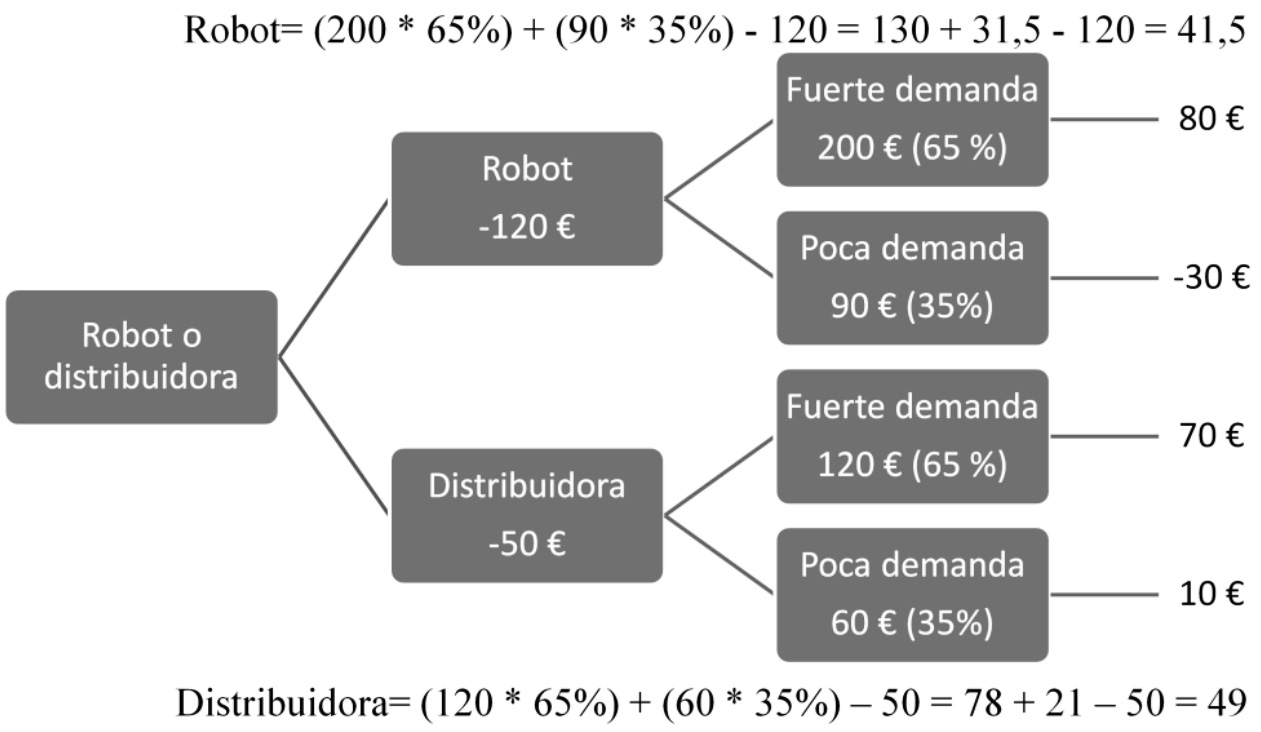
\includegraphics[width=0.7\linewidth]{Resources/emv}
  \caption{EMV de un sistema de clasificación de paquetes.}
  \label{fig:emv}
\end{figure}
    
    
    \item \textbf{Estudio de viabilidad del sistema}:\\
    Pretende determinar si merece la pena la construcción del software: si el sistema puede implantarse con las restricciones de coste y tiempo con la tecnología actual y con un alcance que le sea útil al usuario.\\
    Para ello se hace un estudio de viabilidad desde el punto de vista económico, técnico, legal, operativo y de plazos.
    \begin{figure}[H]
        \centering
        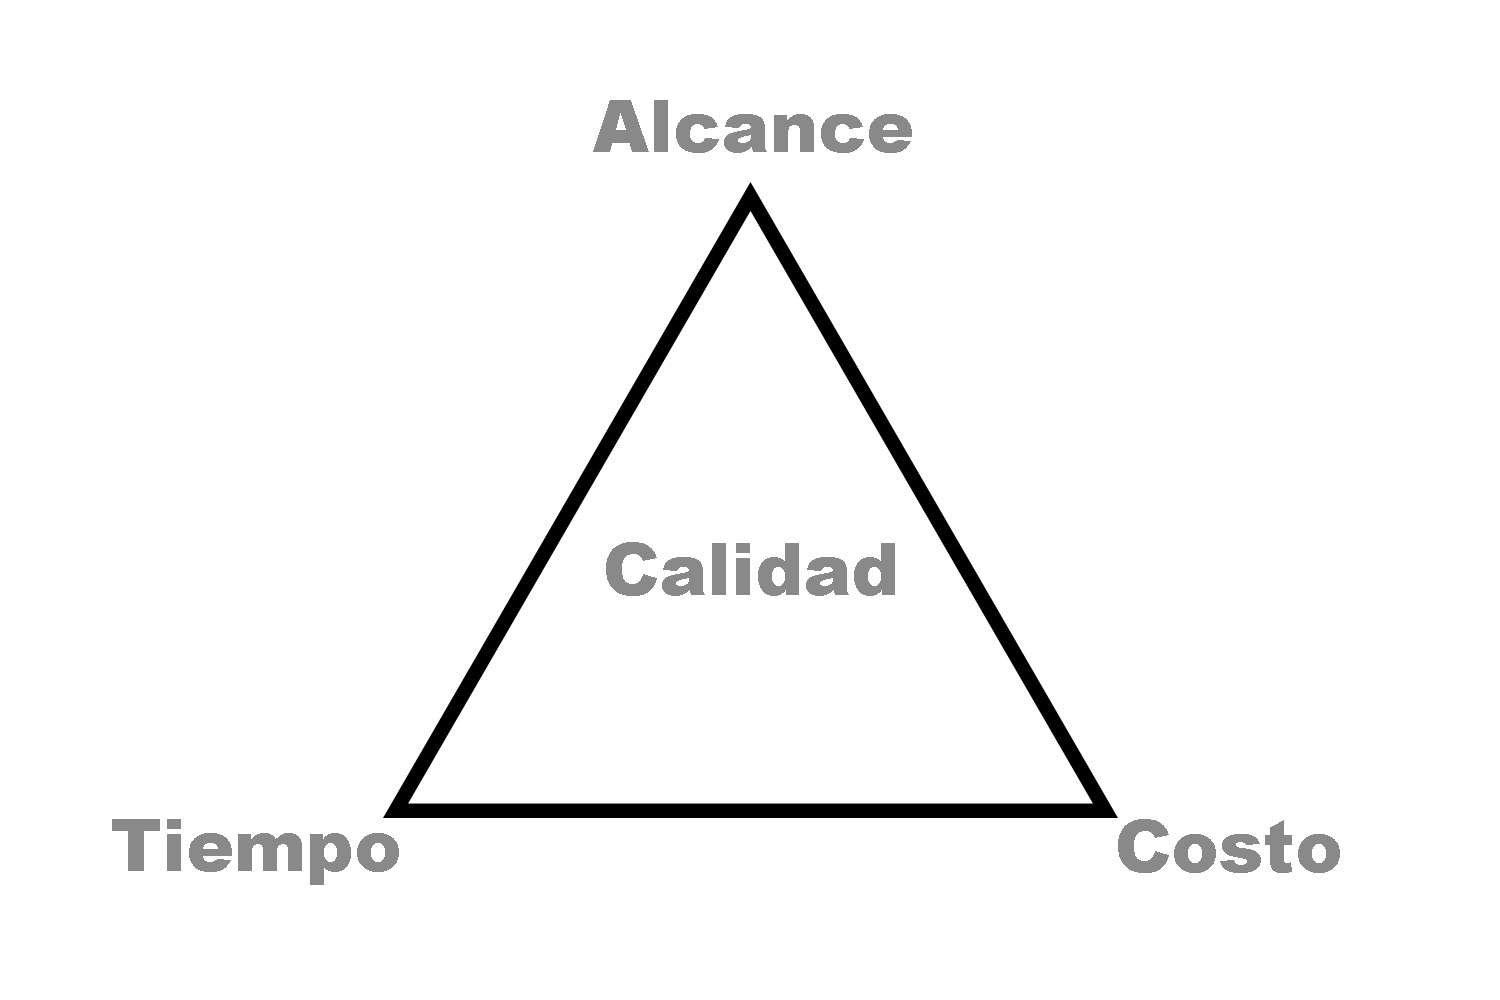
\includegraphics[width=0.4\linewidth]{Resources/PMI}
        \caption{La calidad del software está restringida en mayor medida, pero no únicamente por el tiempo, el coste y el alcance.}
        \label{fig:PMI}
    \end{figure}
    
    \item \textbf{Definición del sistema para que sea la base del trabajo posterior}: Para ello tenemos los siguientes diagramas:
    \begin{itemize}
        \item \textbf{Diagrama de contexto}: Representa el sistema en relación con su entorno. Define los límites del sistema y muestra todos los productores y consumidores de información. El sistema se relaciona con los agentes externos mediante flujos de información.\\
        \textit{Pressman} recomienda realizar este diagrama separado en secciones: Entrada, Salida, interfaz de usuario, función y control de sistema y mantenimiento y diagnóstico.
        \begin{figure}[H]
        \centering
        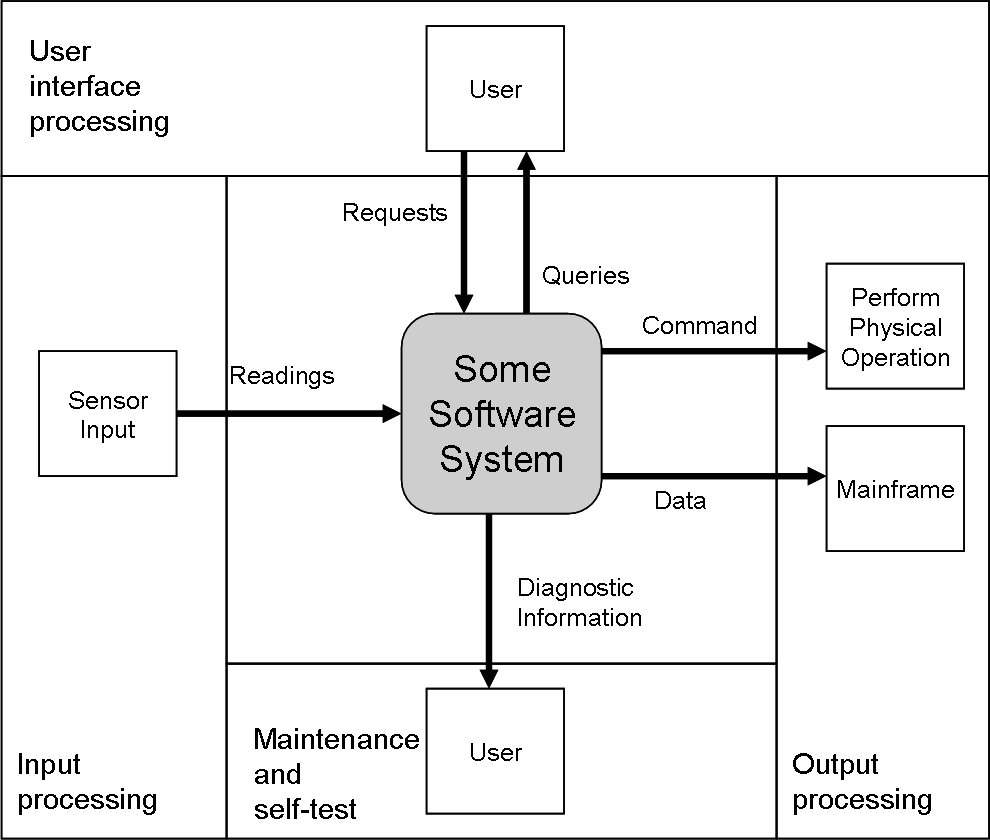
\includegraphics[width=0.5\linewidth]{Resources/contextdiagram}
        \caption{Ejemplo de diagrama de contexto siguiendo la plantilla.}
        \label{fig:diagramaDeContexto}
    \end{figure}
        \item \textbf{Diagrama de flujo}: Determinan el flujo de entre los diferentes subsistemas a través de diagramas de flujo convencionales.
    \end{itemize}
\end{enumerate}.


% Inicio de la zona que o aparece en los apuntes del rabens
\subsection{Análisis de requisitos del software}

El análisis de requisitos del software tiene como objeto\textbf{ desarrollar una representación del software que pueda ser revisada y aprobada por el cliente} que permitirá valorar la calidad del software una vez construido.
\\\\
Desde el punto de vista del analista, esta fase define con mayor precisión las funciones y rendimiento del software, las interfaces con otros componentes y las restricciones que debe cumplir. 

\subsubsection{Principios del análisis de requisitos del software}
\begin{enumerate}
    \item \textbf{Identificar y representar el ámbito de información del sistema}: La tarea que realiza el software consiste en procesar información, representada tanto por \textbf{datos} como por \textbf{sucesos o eventos}. El ámbito de información admite dos puntos de vista: flujo de datos y flujo de control.
    \item \textbf{Modelar la información, la función y el comportamiento del sistema}: Se emplean \textbf{modelos de datos} (información que transforma el software), \textbf{modelos de procesos} (procesos que transforman la información) y \textbf{modelos de control} (comportamiento del sistema).\\
    Utilidades de los modelos:
    \begin{itemize}
        \item Ayudan al analista a entender la información, función y comportamiento del sistema.
        \item Sirven de base para el trabajo del diseñador.
        \item Sirven para validar el producto una vez desarrollado.
    \end{itemize}
    \item \textbf{Descomponer el problema de forma que se reduzca la complejidad.}
    \item \textbf{Avanzar desde lo más general a lo más detallado.}
\end{enumerate}
% Fin de la zona que no aparece en los apuntes del rabenso


\section{Especificación}

\subsection{Especificación del sistema} 
Documento que describe la función, rendimiento y restricciones que el sistema debe cumplir, limitando cada uno de sus componentes.\\

Es labor del analista realizar una \uline{evaluación inicial}, determinando si:
\begin{enumerate}
     \item Se ha delimitado correctamente el ámbito.
     \item Se han definido correctamente las funcionalidades, el comportamiento, las interfaces y el rendimiento.
     \item Las necesidades de usuario y el análisis de viabilidad justifican el desarrollo del proyecto.
     \item Las percepciones acerca del objetivo del proyecto del cliente y el analista coinciden.
\end{enumerate}
El analista deberá hacer además una \uline{evaluación técnica}, comprobando:
\begin{enumerate}
    \item Todos los detalles técnicos están bien definidos.
    \item La especificación sirve como base para las siguientes fases.
    \item Las estimaciones de riesgos, tiempos y costes se corresponden con la complejidad del proyecto.
\end{enumerate}


\subsection{Especificación del software} 
Documento que define, de forma completa, precisa y verificable, los requisitos, el diseño, el comportamiento u otras características de un sistema o componente del mismo.\\
Es el documento que culmina el análisis de requisitos, conteniendo:
\begin{enumerate}
    \item Descripción detallada del ámbito de información.
    \item Funciones y comportamiento asignados al software.
    \item Restricciones de rendimiento y diseño.
    \item Pruebas de aceptación.
\end{enumerate}


% % \subsection{Especificación de requisitos}
% % Documento que define de forma completa, precisa y verificable, los requisitos, el diseño, el comportamiento u otras características del sistema o un componente del mismo.\\\\
% Debe contener una descripción detallada del ámbito de información, las funciones, el comportamiento del software, los requisitos de rendimiento y restricciones de diseño, y sobre las pruebas que se realizarán al software una vez construido.
\subsubsection{Principios de especificación}
\begin{enumerate}
    \item Debe modelar el dominio del problema.
    \item Es necesario separar funcionalidad e implementación.
    \item El lenguaje de especificación debe estar orientado al proceso.
    \item Debe abarcar todo el sistema del que el software es parte.
    \item Debe abarcar también el entorno del sistema.
    \item La especificación debe ser operativa.
\end{enumerate}

\subsubsection{Características del documento de especificación}

\begin{enumerate}
    \item \textbf{Preciso}: Cada requisito debe tener una única interpretación. Evitar el lenguaje natural.
    \item \textbf{Completo}: Una especificación de requisitos software (ERS) está completa si:
    \begin{itemize}
        \item Incluye todos los requisitos significativos del software.
        \item Define la respuesta software a todas las entradas en todas las situaciones.
        \item Está conforme con cualquier estándar de especificación que se deba cumplir.
        \item Están etiquetadas y referenciadas todas las tablas, figuras y diagramas del texto, y están definidos todos los términos y unidades de medida.
        \item No contiene la expresión \textit{TBD} (por determinar). A veces es necesario utilizarla, y debe acompañarse de:
        \begin{itemize}
            \item Una descripción de las condiciones que han causado el \textit{TBD}.
            \item Una descripción de qué hay que hacer para eliminar el \textit{TBD}.
        \end{itemize}
    \end{itemize}
    \item \textbf{Fácil de verificar}. Cualquier requisito al que hace referencia se puede verificar mediante algún procedimiento finito y efectivo en coste.
    \item \textbf{Consistente}: %Se entiende que es la especificación del software porque estamos hablando de eso XD
    \begin{itemize}
        \item Ningún conjunto de requisitos descritos en la especificación deben describir el mismo objeto real pero utilizar distintos términos para designarlo.
        \item Las características especificadas de objetos reales no pueden estar en conflicto.
        \item Ningún conjunto de acciones determinadas deben entrar en conflicto lógico o temporal.
    \end{itemize}
    \item \textbf{Fácil de modificar}.

    \item \textbf{Facilidad para identificar el origen y las consecuencias de cada requisito}: se consigue estableciendo la trazabilidad.
    
    \item \textbf{Facilidad de utilización durante la fase de explotación y mantenimiento}. %osea el REM no

\end{enumerate}





\section{Verificación y Validación de requisitos}
\subsection{Estrategias}
Encontramos diferentes estrategias para la verificación y validación de requisitos:
\begin{enumerate}
    \item \textbf{Comprobación de validez}. ¿Responde a todas las necesidades?
    \item \textbf{Comprobación de consistencia}. ¿Hay incongruencias en los requisitos? % XD
    \item \textbf{Comprobación de totalidad}. ¿Nos falta algo por especificar? 
    \item \textbf{Verificaciones de realismo}. ¿Es posible implementar la funcionalidad requerida?
    \item \textbf{Verificabilidad}. ¿Soy capaz de crear pruebas que determinen si se pasa cada requisito?
\end{enumerate}

\subsection{Técnicas}
Existen varias \uline{técnicas de validación} de requisitos:

\begin{enumerate}
    \item \textbf{Revisiones de requisitos} Proceso manual de verificación del documento de requisitos que busca encontrar anomalías y omisiones.%por grupos de revisores %Los requisitos son analizados por un grupo de revisores.
    \item \textbf{Construcción de prototipos}. %Se muestra un modelo ejecutable del sistema a los usuarios finales para que experimenten con él.
    \item \textbf{Generación de casos de prueba}. Los requisitos deben poder probarse. Si una prueba es difícil o imposible de diseñar, suele significar que los requisitos serán difíciles de implementar, por lo que deben ser reconsiderados.
    \item \textbf{Análisis de consistencia automática}. Si los requisitos se expresan como un modelo del sistema en una notación estructurada o formal, las herramientas CASE(Computer Aided Software Engineering) deben verificar la consistencia del modelo.
\end{enumerate}
% aparte esta arriba
% Estaba en el enumerate mencionado (porque así lo tiene rabenso), no creo que quiera que sepamos mucho del tema hay bastantes más cosas importantes que las clasificaciones de las revisiones de requisitos/
\section{Administración de requisitos}
La especificación de requisitos es un proceso iterativo, por lo tanto hace falta un proceso formal para gestionar la realización de modificaciones a los requisitos sin descuidar la calidad de la documentación de requisitos.\\
Para ello debemos llevar a cabo un registro de modificaciones

\subsection{Clasificación cualitativa}
\begin{enumerate}
    \item \textbf{Requisitos duraderos}
    \item \textbf{Requisitos volátiles}
    \begin{itemize}
        \item \textbf{Cambiantes}: Cambian debido a los cambios en el ambiente en que opera la organización. 
        \item \textbf{Emergentes}: Surgen al incrementar la comprensión del cliente en el desarrollo del sistema.
        \item \textbf{Consecutivos}: Son resultado de la introducción del sistema de cómputo. %valla nombre de mierda
        \item \textbf{De compatibilidad}: Dependen de sistemas particulares o procesos de negocio dentro de la organización.
    \end{itemize}
\end{enumerate}
\subsection{Clasificación cuantitativa}
Asignándole un valor de estabilidad(baja, media y alta).

\subsection{Etapas}
El proceso de administración de requisitos tiene dos etapas:

\begin{enumerate}
    \item \textbf{Planificación}:\\
    En esta etapa debemos de decidir el nivel de detalle estableciendo:
    \begin{enumerate}[a.]
        \item \textbf{La identificación de requisitos}.
        \item \textbf{Un proceso de administración del cambio}.
        \item \textbf{Políticas de rastreo}: Requisito -- Fuente, Requisito -- Requisito, y Requisito -- Diseño.
        %Imagen de politica de rastreo
        \item \textbf{Ayuda de herramientas CASE}: Etablecemos las herramienta de \textbf{C}omputer \textbf{A}ided \textbf{S}oftware \textbf{E}ngineering que utilizaremos para aumentar la productividad durante el desarrollo.
    \end{enumerate}
    
    \item \textbf{Administración del cambio}:\\
    Se aplica para todos los cambios en los requisitos, teniendo las siguientes sub--etapas:
        \begin{enumerate}[a.]
        \item \textbf{Análisis del problema y especificación del cambio}.
        \item \textbf{Análisis del cambio y costeo}.
        \item \textbf{Implementación del cambio}.
\end{enumerate}
    
\end{enumerate}

%Ale tema acabado